\documentclass[12pt]{article}
\usepackage[T2A]{fontenc}
\usepackage[utf8]{inputenc}
\usepackage{multirow}
\usepackage{caption}
\usepackage{subcaption}
\usepackage{amsmath}
\usepackage{changepage}
\usepackage{graphicx}
\usepackage{float}
\usepackage[english,russian]{babel}
\usepackage{amsmath, amsfonts, amssymb, amsthm, mathtools}
\usepackage{xcolor}
\usepackage{array}
\usepackage{hyperref}
\usepackage{icomma}
\usepackage{mathtext} 
\usepackage[top = 1.5cm, left = 1.5 cm, right = 1.5 cm, bottom = 3 cm]{geometry}
\graphicspath{ {./images/} }
 
\title{Плазма. Газовый разряд}
\author{Шахматов Андрей, Б02-304}
\date{\today}
  
\begin{document}
\begin{titlepage}
	\begin{center}
		{\large МОСКОВСКИЙ ФИЗИКО-ТЕХНИЧЕСКИЙ ИНСТИТУТ (НАЦИОНАЛЬНЫЙ ИССЛЕДОВАТЕЛЬСКИЙ УНИВЕРСИТЕТ)}
	\end{center}
	\begin{center}
		{\large Физтех-школа физики и исследований им. Ландау}
	\end{center}

	\vspace{3cm}
	{\huge
		\begin{center}
			\textbf{Плазма. Газовый разряд}
		\end{center}
	}
	\vspace{2cm}
	\begin{flushright}
		{\LARGE Автор:\\ Шахматов Андрей Юрьевич \\
			\vspace{0.2cm}
			Б02-304}
	\end{flushright}
	\vspace{7 cm}
	\begin{center}
		Долгопрудный 2024
	\end{center}
	\thispagestyle{empty}
\end{titlepage}

% \maketitle

\begin{abstract}
	Исследованы характеристики плазмы в тлеющем газовом разряде. Получена вольт - амперная
	характеристика плазмы. При помощи двойного зонда определены характеристики плазмы:
	плазменная частота колебаний электронов и дебаевский радиус экранирования. Определено,
	что плазма в тлеющем газовом разряде хорошо описывается моделью идеальной плазмы.
\end{abstract}

% \tableofcontents

\section*{Введение}
Цель работы заключается в исследовании характеристик плазмы телющего газового разряда при помощи двойного зонда.

\section*{Методика}
\subsection*{Основные характеристики плазмы}
Определяющими свойвствами плазмы являются коллективный характер её движения и квазинейтральность (равенство нулю средней плотности заряда).
Таким образом можно рассмотреть коллективные колебания плазмы относительно квазинейтрального состояния.
Для этого выделим в нейральной плазме некоторый объём в виде параллелепипеда.
При перемещении всех электронов на расстояние $x$ относительно ионов на боковых гранях образуются нескомпенсированные
поверхностные заряды с плотностью
\[
	\sigma = \pm n_e e \Delta x.
\]
Эти заряды создадут электрическое поле
\[
	E = 4\pi n_e e \Delta x .
\]
В таком случае можно записать уравнение колебаний
\[
	\frac{d^2 x}{dt^2} = -\frac{eE}{m} = -\frac{4\pi n_e e^2}{m} \Delta x .
\]
В таком случае плазменная частота гармонических колебаний будет выражаться как
\begin{equation}
	w_p = \sqrt{\frac{4\pi n_e e^2}{m_e}}.
	\label{eq:1}
\end{equation}

Также можно ввести характерный размер плазменных явлений как отношение тепловой скорости частиц к плазменной частоте
\begin{equation}
	r_D = \sqrt{\frac{k_B T_e}{4\pi n_e e^2}},
	\label{eq:2}
\end{equation}
где величину $r_D$ называют Дебаевским радиусом. Также можно показать, что дебаевский радиус является характерным радиусом экранирования
действия заряженной частицы на другие частицы. В таком случае потенциал частицы будет иметь вид
\[
	\varphi(r) = \frac{q}{r} e^{-\frac{r}{r_D}}.
\]
\subsection*{Одиночный зонд}
При внесении в плазму уединённого проводника --- \textit{зонда} --- с потенциалом, изначально равным потенциалу точки плазмы, в которую его помещают, на него поступают токи электроннов и ионов:
\[
	I_{e0} = \dfrac{n \langle v_e \rangle}{4}eS,
\]
\[
	I_{i0} = \dfrac{n \langle v_i \rangle}{4}eS,
\]
где $\langle v_e \rangle$ и $\langle v_i \rangle$ --- средние скорости электронов и ионов,
$S$ --- площадь зонда, $n$ --- плотность электронов и ионов.
Скорости электронов много больше скорости ионов,
поэтому $I_{i0} \ll I_{e0}$.
Зонд будет заряжаться до некоторого равновестного
напряжения $-U_f$ --- \textit{плавающего потенциала}.\\
В равновесии ионный ток мало меняется, а электронный имеет вид
$$
	I_e = I_0 \exp\left( -\dfrac{eU_f}{kT_e} \right).
$$
Будем подавать потенциал $U_\text{з}$ на зонд и снимать значение зондового тока $I_\text{з}$.
Максимальное значение тока $I_{e\text{н}}$ --- электронный ток насыщения, а минимальное $I_{i\text{н}}$ --- ионный ток насыщения. Значение из эмпирической формулы Бомона:
\[
	I_{i\text{н}} = 0.4 neS \sqrt{\dfrac{2kT_e}{m_i}}.
\]
Электронный ток насыщения можно определить по тепловому движению:
\[
	I_{e\text{н}} = \frac{n_eS}{4}\sqrt{\frac{8kT}{\pi m_e}}.
\]

\subsection*{Двойной зонд}
Двойной зонд --- система из двух одинаковых зондов, расположенных на небольшом расстоянии друг от друга, между которыми создаётся разность потенциалов, меньшая $U_f$. Рассчитаем ток между ними вблизи $I=0$. При небольших разностях потенциалов ионные токи на оба зонда близки к току насыщения и компенсируют друг друга, а значит величина результирующего тока полностью связана с разностью электронных токов. Пусть потенциалы на зондах
$$
	U_1 = -U_f + \Delta U_1,
$$
$$
	U_2 = -U_f + \Delta U_2.
$$
Между зондами $U = U_2 - U_1 = \Delta U_2 - \Delta U_1$.
Через первый электрод
\[
	I_1 = I_{i\text{н}} + I_{e1} = I_{i\text{н}} - \dfrac{1}{4}neS\langle v_e\rangle \exp\left(-\dfrac{eU_f}{kT_e}\right)\exp\left(\dfrac{e\Delta U_1}{kT_e}\right)=I_{i\text{н}}\left(1 - \exp\left( \dfrac{e\Delta U_1}{kT_e} \right)\right).
\]
Аналогично через второй получим
\[
	I_2 = I_{i\text{н}}\left(1 - \exp\left( \dfrac{e\Delta U_2}{kT_e} \right)\right).
\]

С учётом последовательного соединение зондов ($I_1 = -I_2 = I)$:
$$
	\Delta U_1= \dfrac{kT_e}{e}\text{ln}\left(1 - \dfrac{I}{I_{i\text{н}}}\right),
$$
$$
	\Delta U_2= \dfrac{kT_e}{e}\text{ln}\left(1 + \dfrac{I}{I_{i\text{н}}}\right).
$$

Тогда итоговые формулы для разности потенциалов и тока

\begin{equation}
	U = \dfrac{kT_e}{e}\text{ln}\dfrac{1 - I/I_{i\text{н}}}{1 + I/I_{i\text{н}}}, \ \
	I = I_{i\text{н}} \text{th}\dfrac{eU}{2kT_e}.
	\label{eq:3}
\end{equation}

\begin{figure}[H]
	\centering
	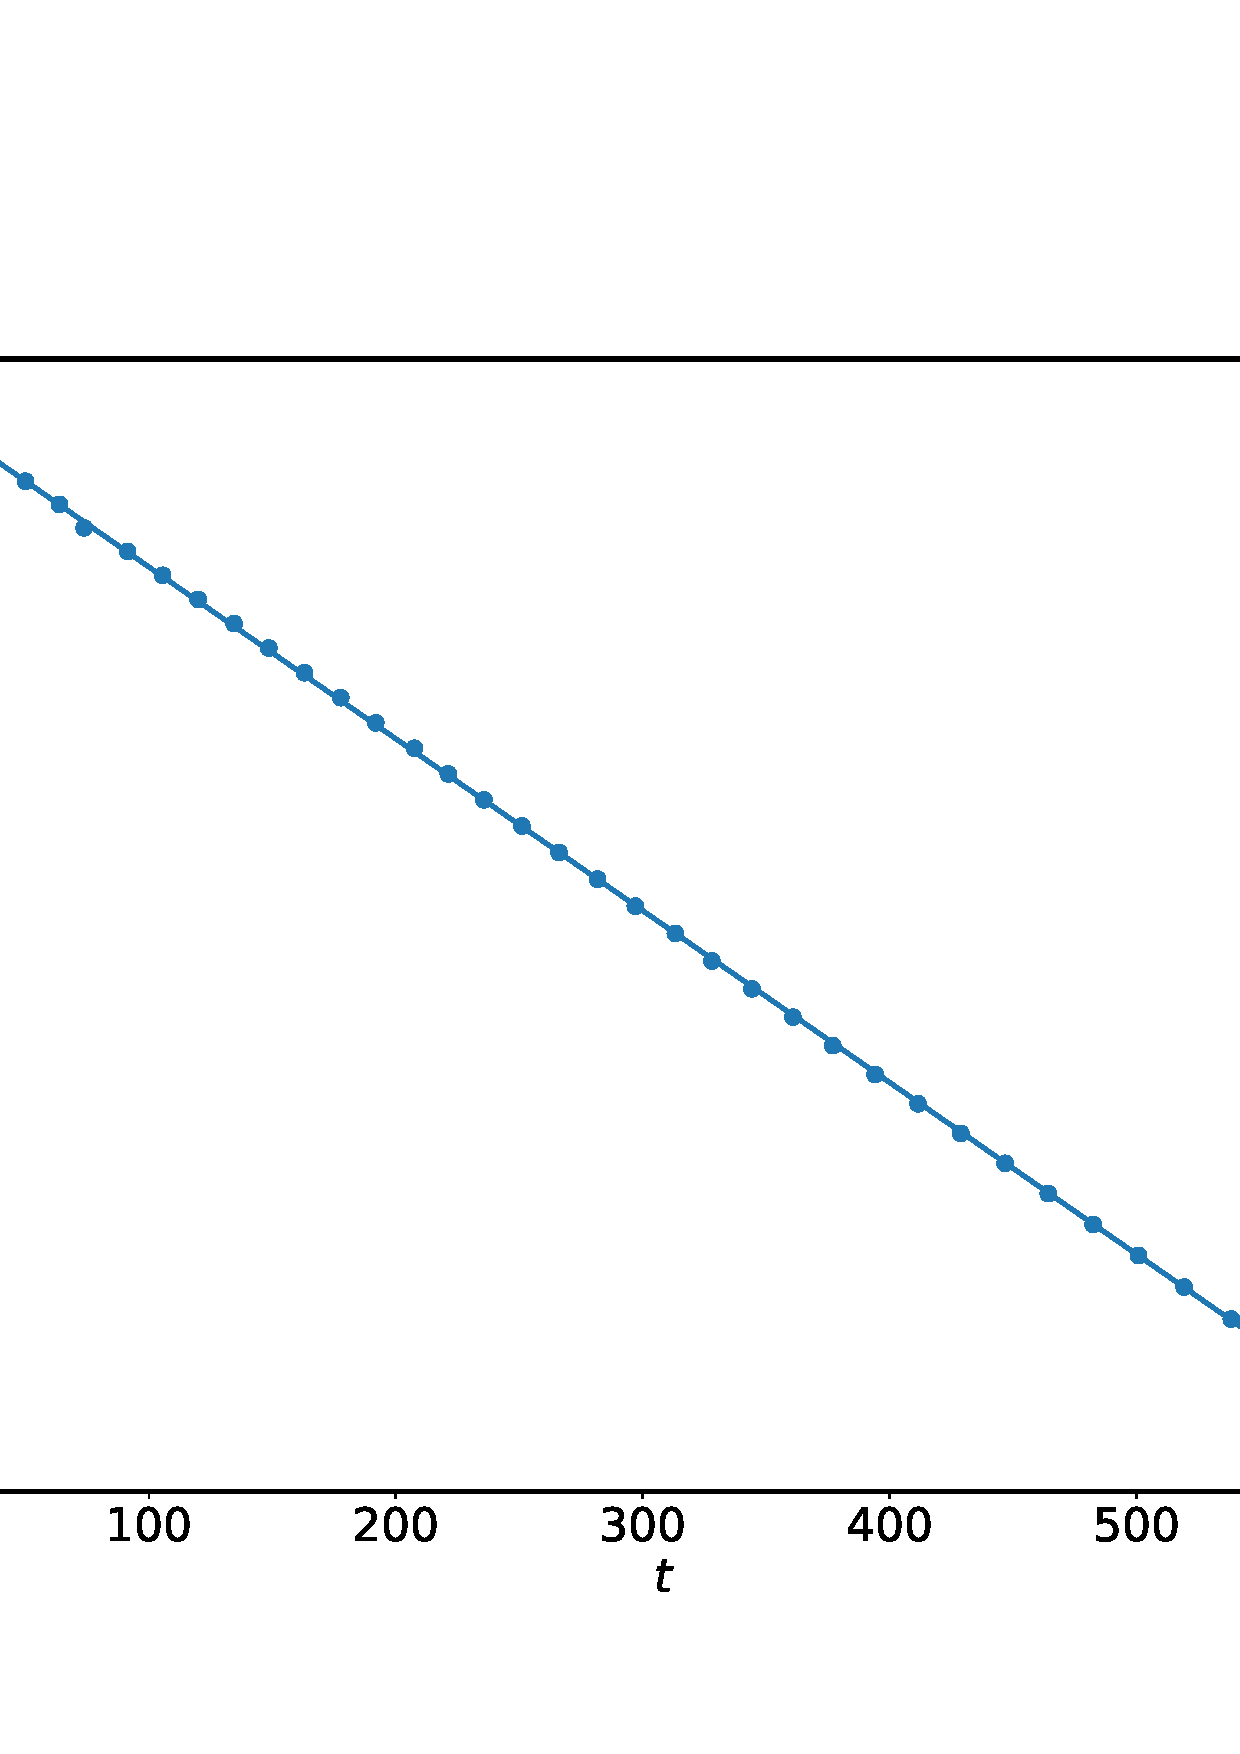
\includegraphics[width=0.5\textwidth]{4.png}
	\caption{Экпериментальный вид зависимости тока $I$ от напряжения $U$ на двойном зонде
	}
	\label{pic:graph}
\end{figure}
Зависимость выглядит как показано на \ref{pic:graph}.
Из формулы можно найти формулу для $T_e$: для $U=0$ мы найдём $I_{i\text{н}}$, продифференцируем в точке $U=0$ и с учётом $\text{th}~\alpha \approx \alpha$ при малых $\alpha$ и $A\rightarrow 0$ получим:
\begin{equation}
	kT_e = \dfrac{1}{2}\dfrac{eI_{i\text{н}}}{\dfrac{dI}{dU}|_{U=0}}.
\end{equation}

\subsection*{Описание установки}
\begin{figure}[H]
	\centering
	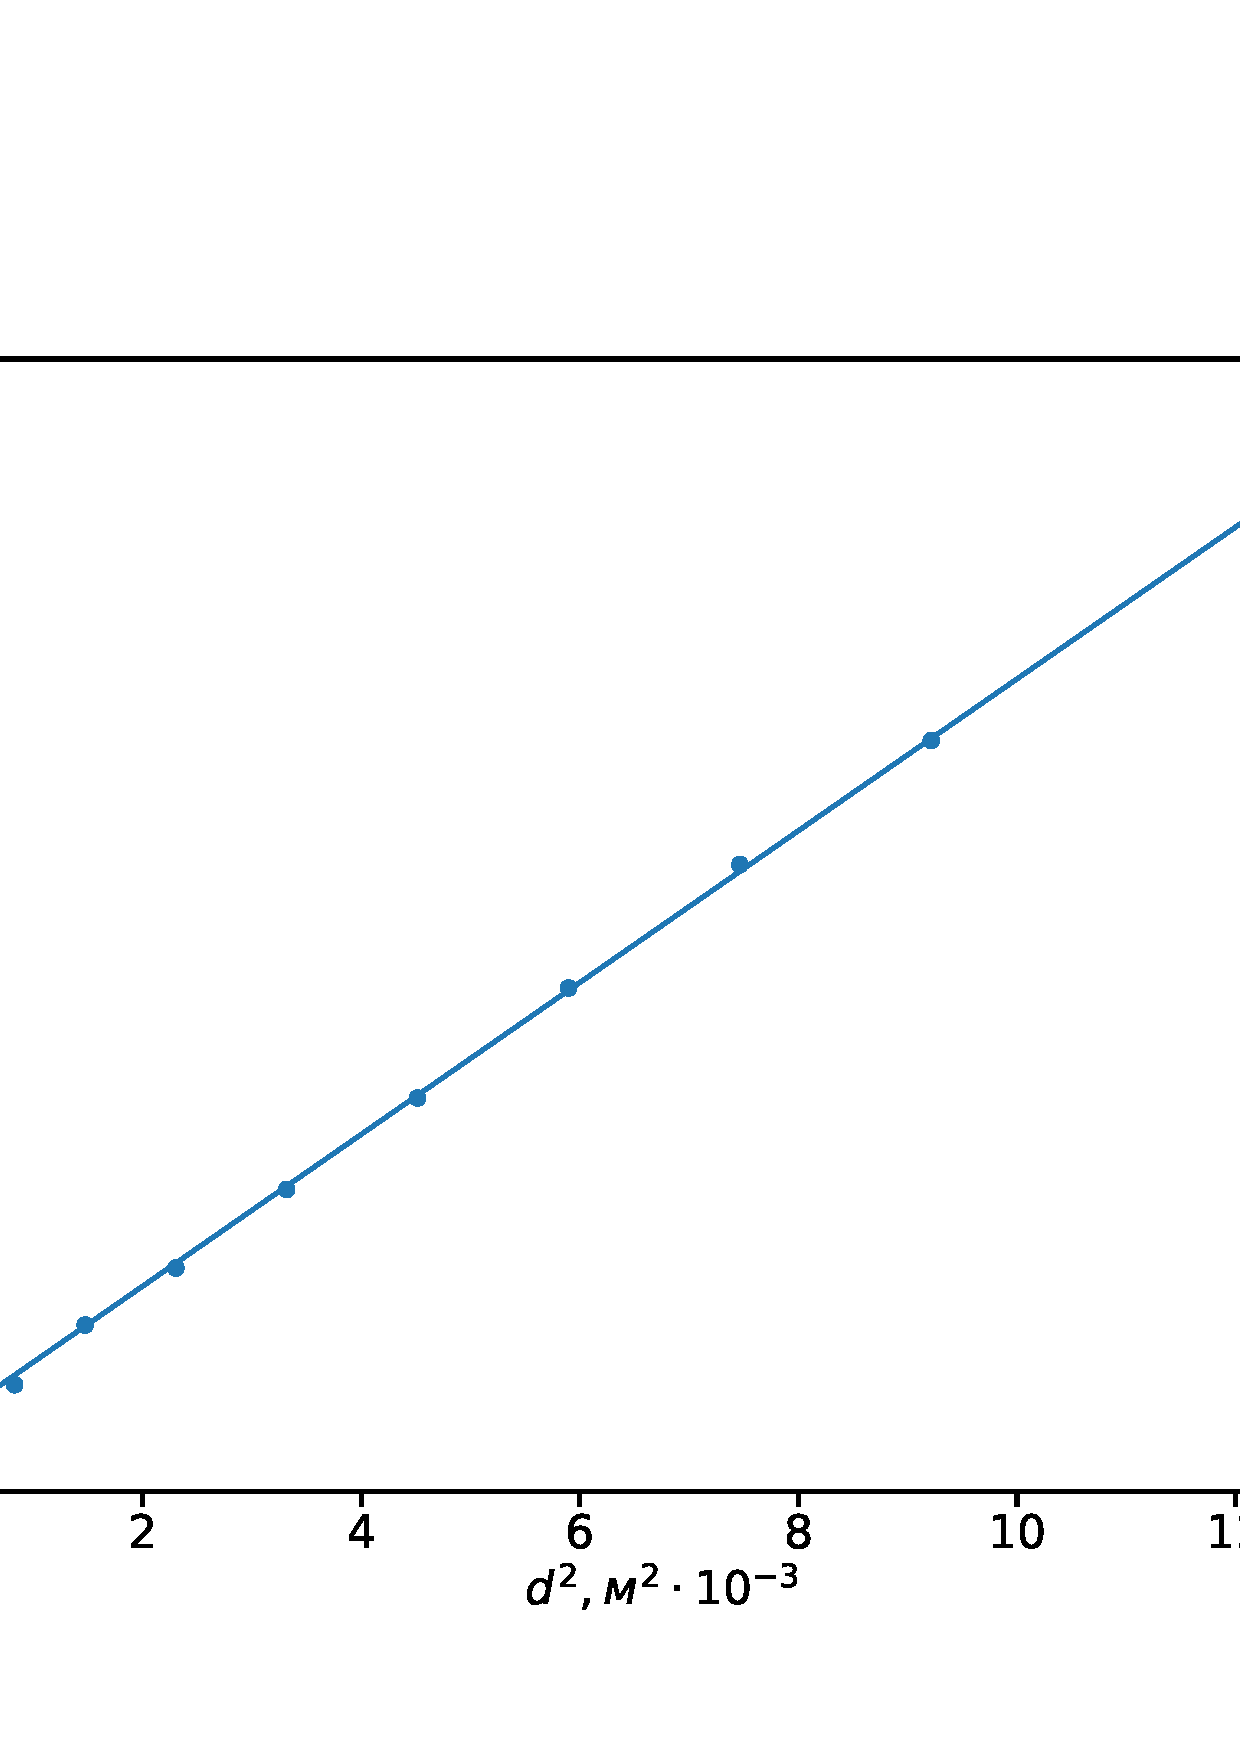
\includegraphics[width=0.6\textwidth]{1.png}
	\caption{Схема установки}
	\label{pic:scheme}
\end{figure}
Стеклянная газоразрядная трубка имеет холодный (ненакаливаемый) полый катод, три анода и \textit{геттерный} узел -- стеклянный баллон, на внутреннюю повехность которого напылена газопоглощающая плёнка (\textit{геттер}). Трубка наполнена изотопом неона $^22$Ne при давлении 2 мм рт. ст. Катод и один из анодом (I и II) с помощью переключателя $\Pi_1$ подключается через балластный резистор $R_\text{б}$ ($\approx 450$ кОм) к регулируемому ВИП с выкодным напряжением до 5 кВ.\\
При подключении к ВИП анода-I между ним и катодом возникает газовый разряд. Ток разряда измеряется миллиамперметром $A_1$, а падение напряжения на разрядной трубке -- цифровым вольтметром $V_1$, подключённым к трубке черезе высокоомный (25 МОм) делитель напряжения с коэффициентом $(R_1+R_2)/R_2 = 10$.\\
При подключении к ВИП анода-II разряд возникает в пространстве между катодом и анодом-II, где находятся двойной зонд, используемый для диагностики плазмы положительного столба. Зонды изготовлены из молибденовой проволоки диаметром $d = 0.2$ мм и имеют длину $l = 5.2$ мм. Они подключены к источнику питания GPS через потенциометр $R$. Переключатель $\Pi_2$ позволяет изменять полярность напряжения на зондах. Величина напряжения на зондах изменяеься с помощью дискретного переключателя <<$V$>> выходного напряжения источника питания и потенциометра $R$, а измеряется цифровым вольтметром $V_2$. Для измерения зондового тока используется мультиметр $A_2$.

\section*{Результаты и их обсуждение}
Измерено напряжение зажигания разряда $U = 267$ В.
проведено измерение вольт-амперной характеристики, данные представлены
в таблице \ref{tab:1}.
\begin{table}[H]
	\centering
	\begin{tabular}{|l|l|l|l|l|l|l|l|l|l|l|l|}
		\hline
		$U$, В  & 260,0 & 251,0 & 250,0 & 237,0 & 225,0 & 207,0 & 180,0 & 167,0 & 145,0 & 120,0 & 104,0 \\ \hline
		$I$, мА & 1,63  & 1,81  & 2,00  & 2,22  & 2,40  & 2,61  & 2,81  & 3,00  & 3,21  & 3,40  & 3,62  \\ \hline
		$U$, В  & 94,5  & 102,6 & 117,0 & 141,0 & 163,0 & 178,0 & 211,0 & 220,0 & 228,0 & 237,0 & ~     \\ \hline
		$I$, мА & 3,80  & 3,60  & 3,40  & 3,21  & 3,00  & 2,80  & 2,60  & 2,40  & 2,20  & 2,00  & ~     \\ \hline
	\end{tabular}
	\caption{Данные зависимости тока через газовый разряд $I$ от напряжения между электродами $U$.}
	\label{tab:1}
\end{table}

Построен график вольт-амперной характеристики (Рис. \ref{fig:UpIp}). С его помощью определено максимальное дифференциальное
сопротивление $R_{\text{дифф}} \approx 1,0 \cdot 10^5$ Ом.
\begin{figure}[H]
	\centering
	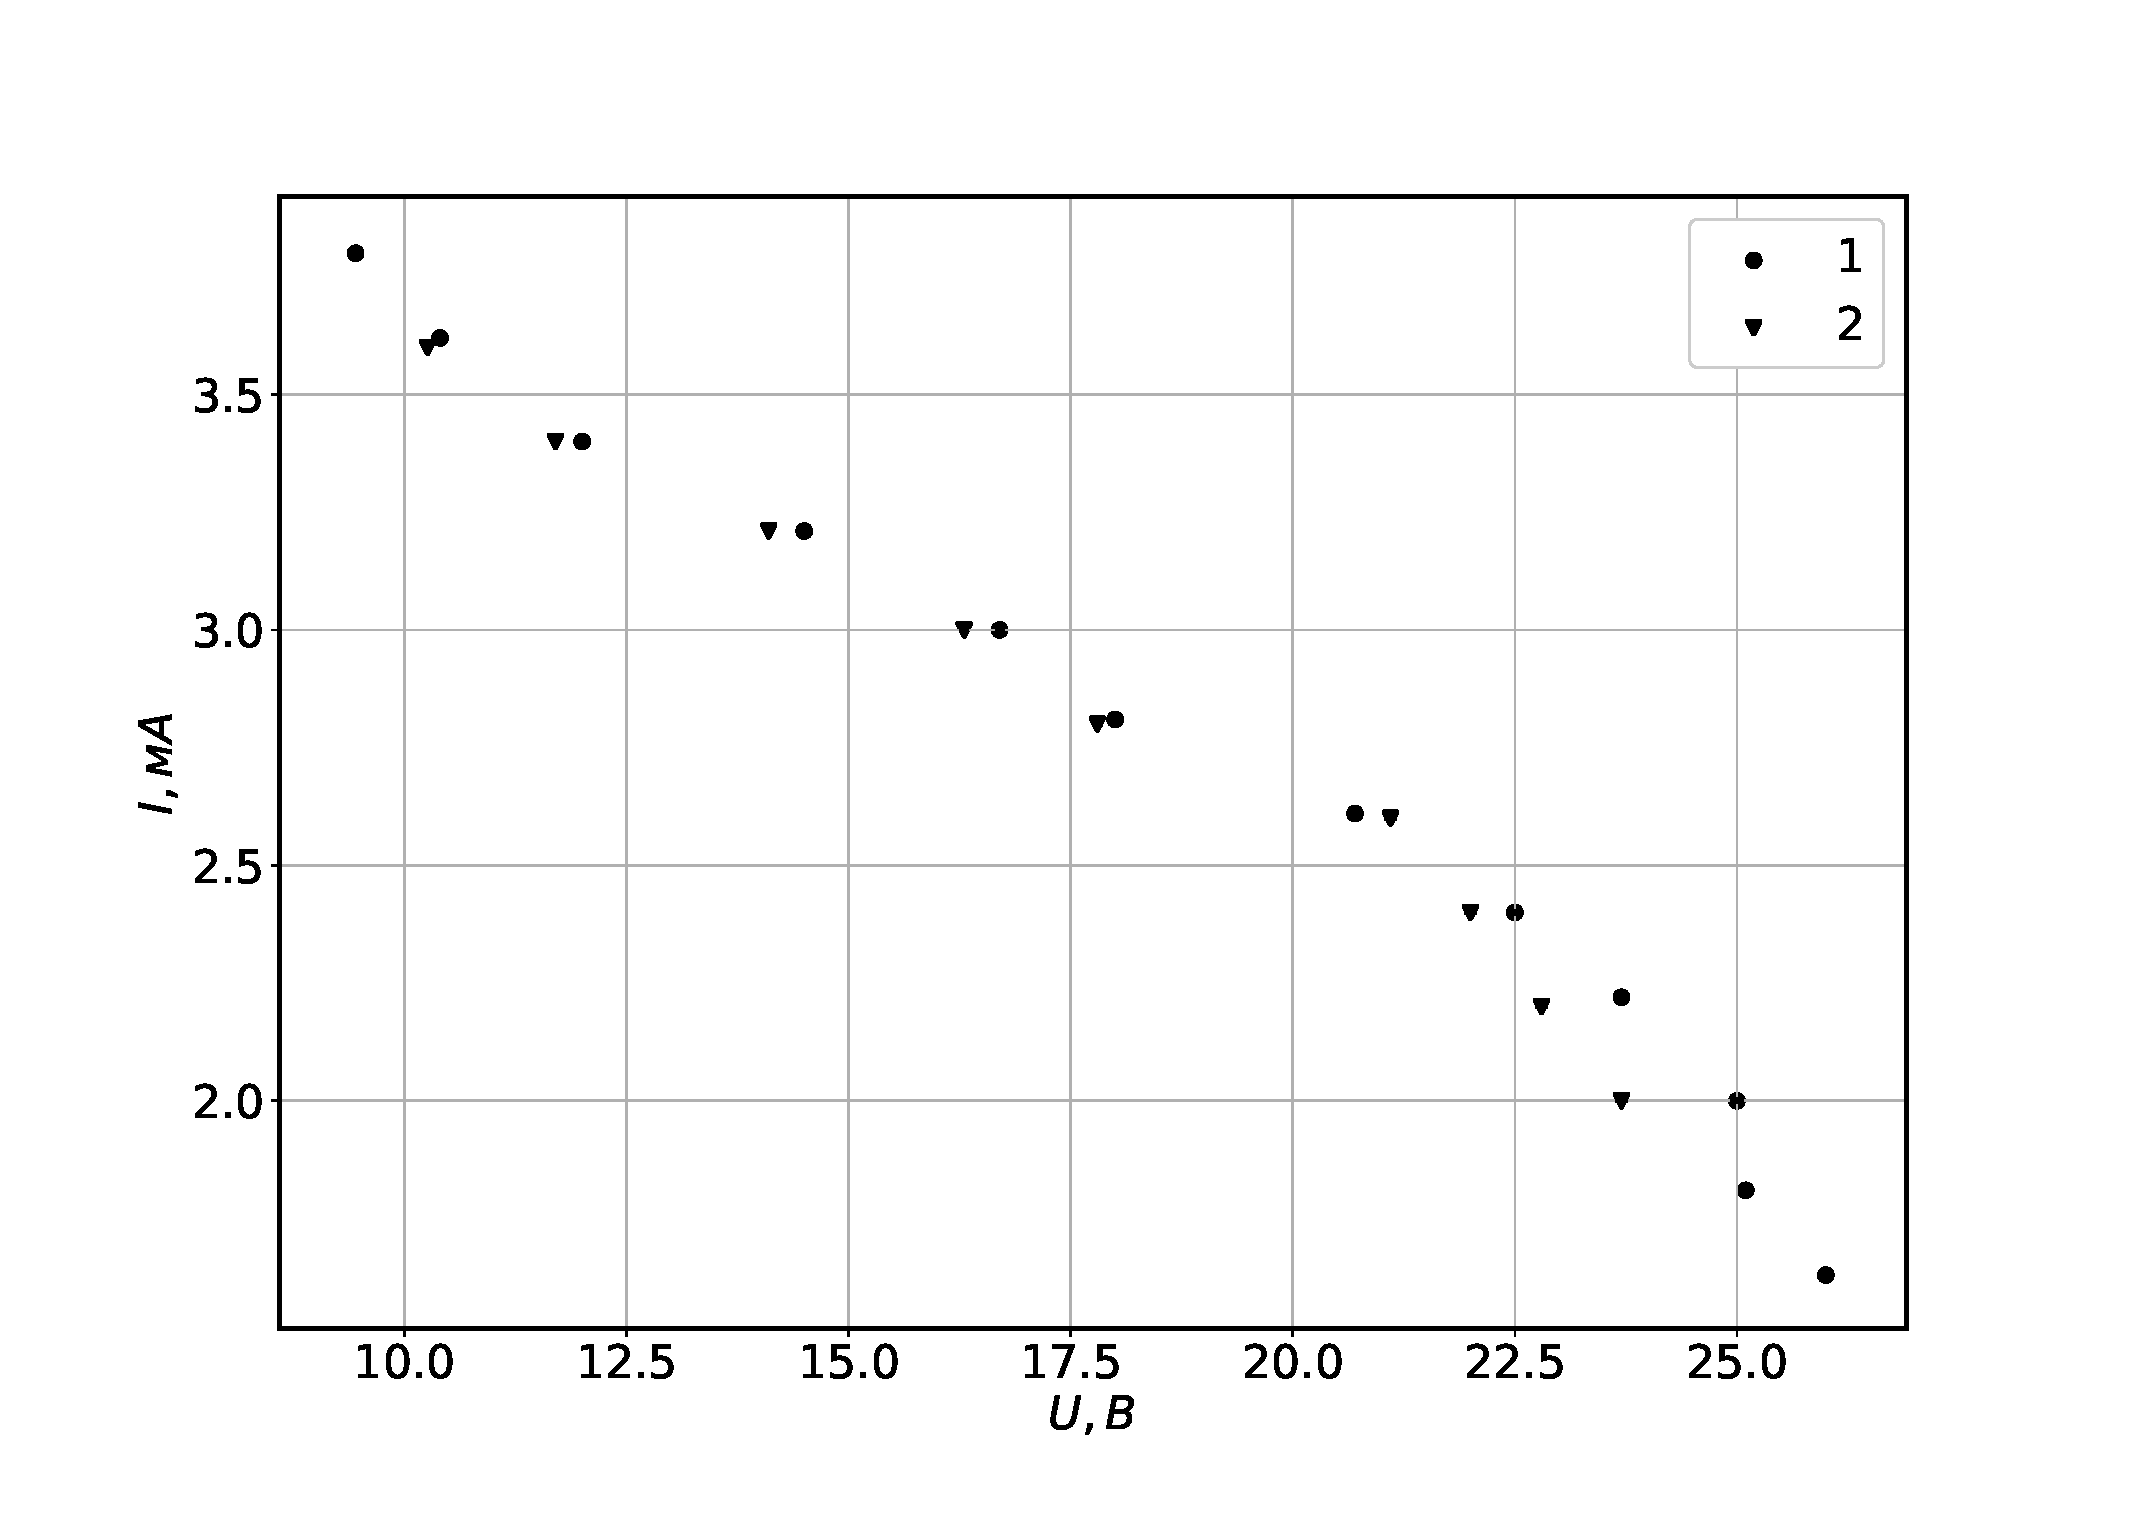
\includegraphics[width=0.8\textwidth]{UpIp.eps}
	\caption{График зависимости тока через газовый разряд $I$ в зависимости от напряжения между электродами $U$.
		Цифрами обозначены 1 --- прямой ход измерений, 2 --- обратный ход измерений.}
	\label{fig:UpIp}
\end{figure}
С помощью амперметра $A_2$  и вольтметра $V_2$ снята зависимость тока от напряжения на двойном зонде в зависимости от тока в газовом
разряде (Таблица \ref{tab:2}).
После центрирования графиков построены соответсвующие зависимости (Рис. \ref{fig:UI}).

\begin{figure}[H]
	\centering
	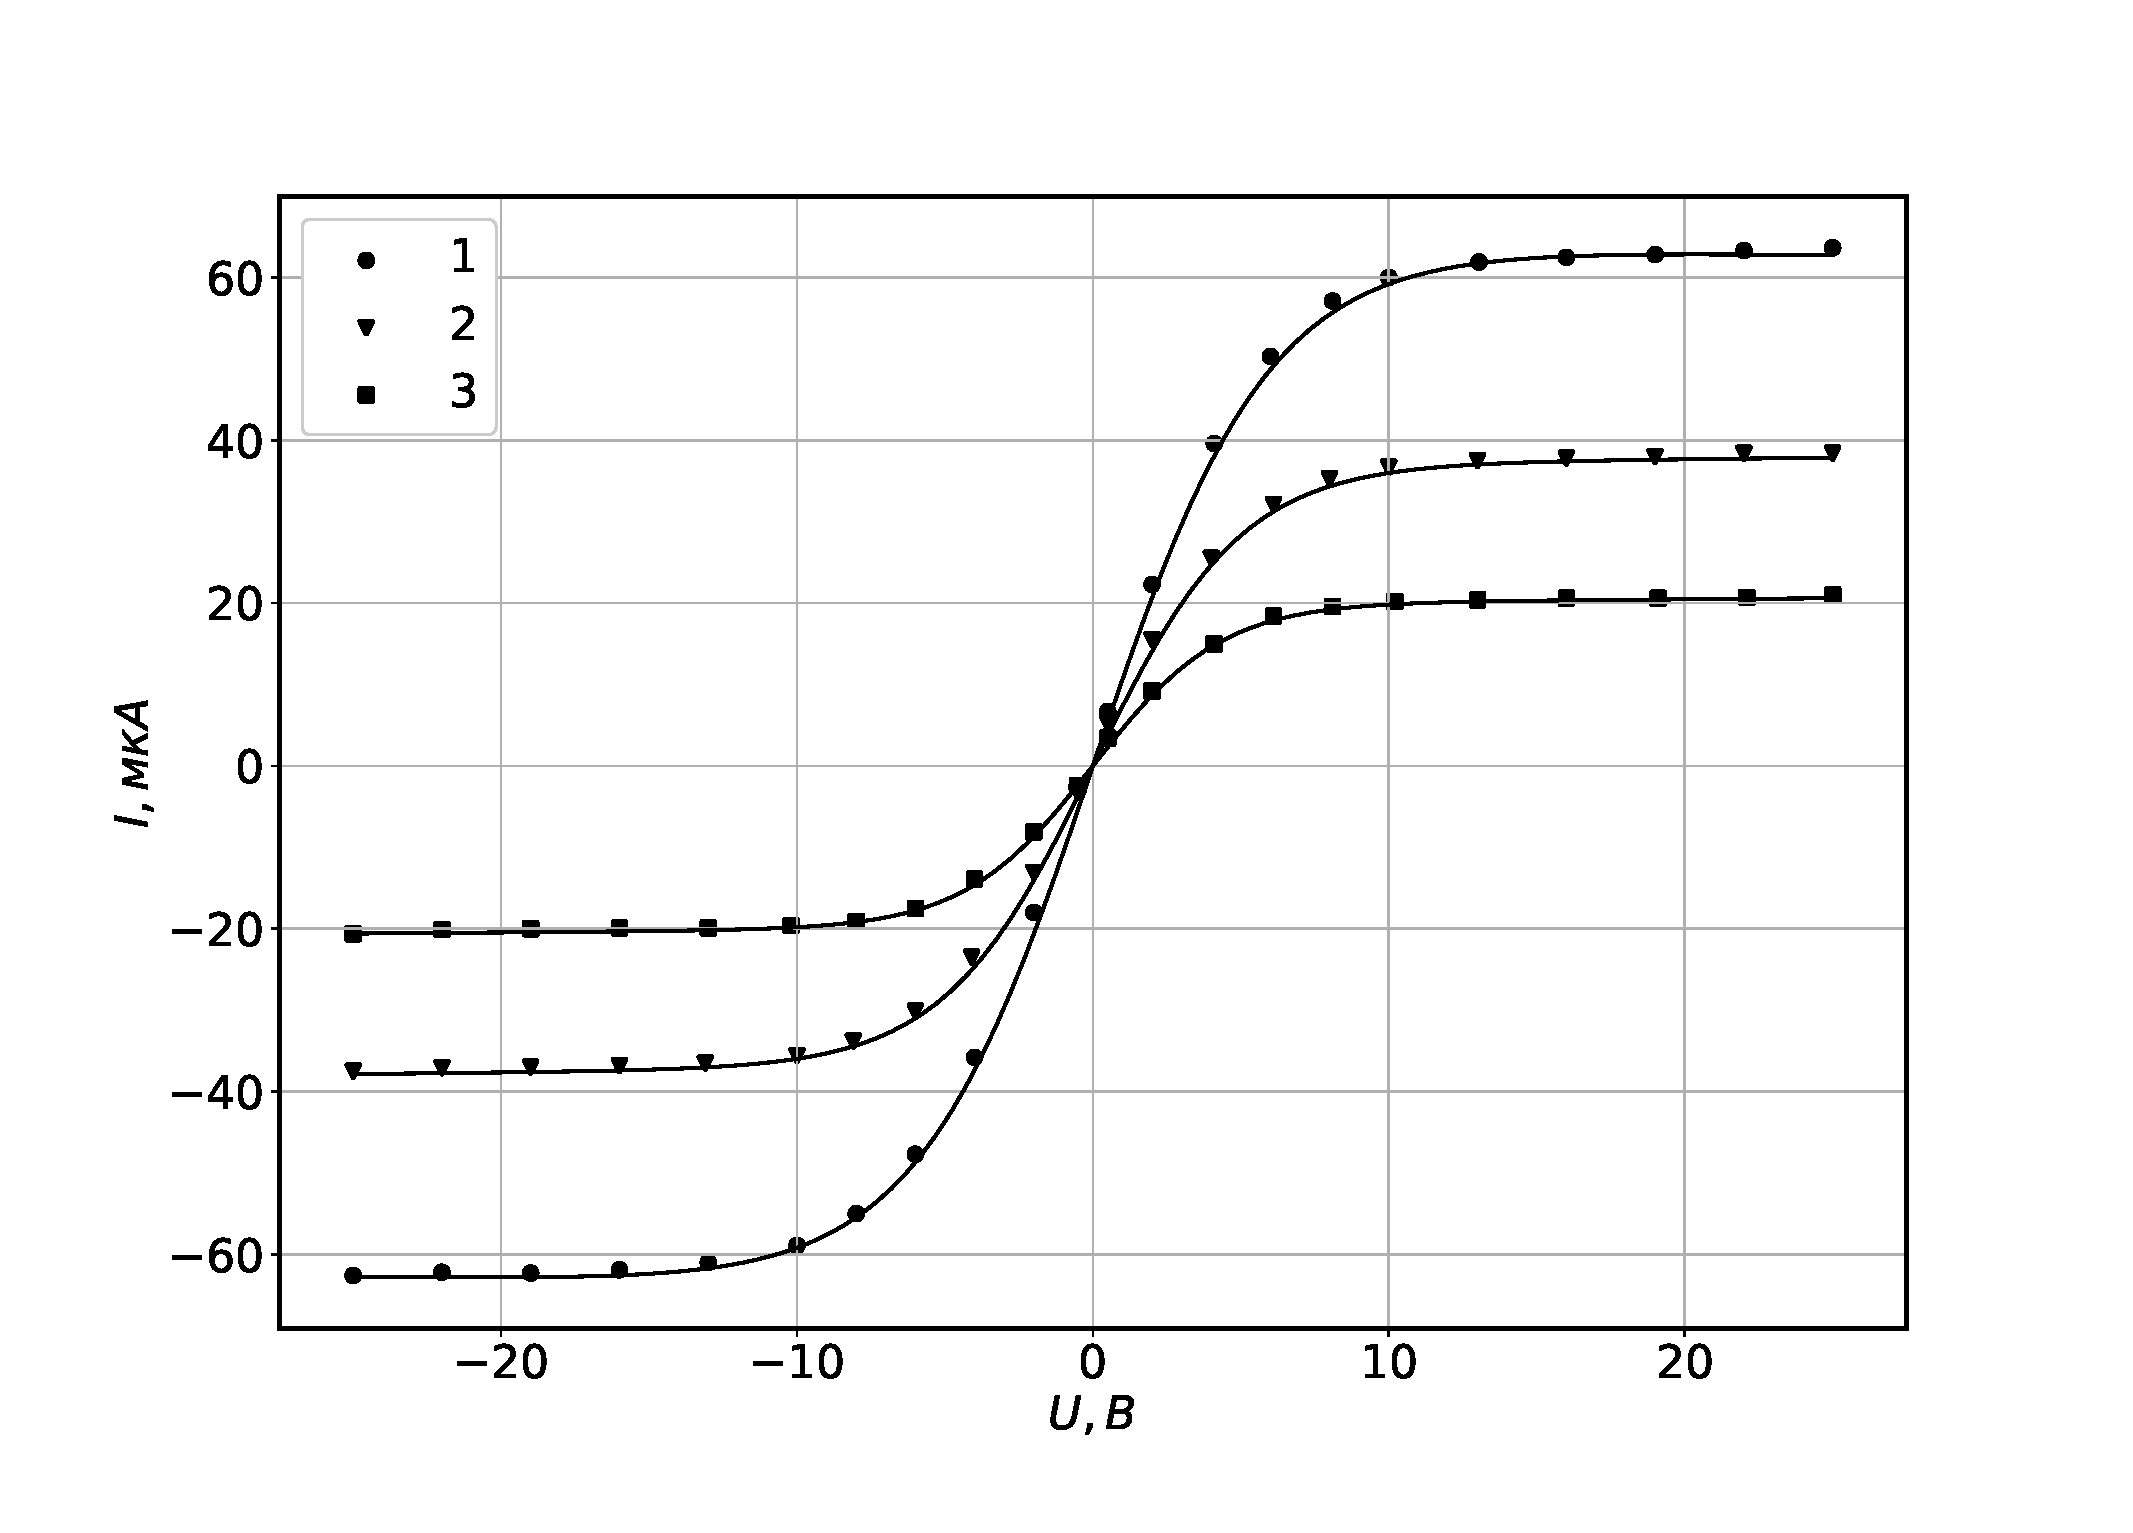
\includegraphics[width=0.8\textwidth]{UI_main.eps}
	\caption{Графики зависимости тока через двойной зонд $I$ от напряжение на зонде $U$.
		Цифрами обозначены графики соответсвующие токам через газовый разряд 1 --- $4,25$ мА,
		2 --- $3,01$ мА, 3 --- $2,04$ мА.}
	\label{fig:UI}
\end{figure}

Проводя ассимптоты г графиками при $U \to \infty$, найдены значения токов насыщения.
Проводя касательную к графику при $U = 0$ В, найдены температуры электронов. После чего согласно
выражениям \ref{eq:1}, \ref{eq:2} найдены дебаевский радиус $r_D$ и ленгморовская частота $w_p$.
Рассчитанные значения представлены в таблице \ref{tab:3}.
\begin{table}[H]
	\centering
	\begin{tabular}{|l|l|l|l|l|l|l|l|l|}
		\hline
		$I$, мА         & $I_{i\text{н}}$, мкА & $T_e$, К         & $n_e$, $10^{16} \cdot \text{м}^{-3}$ & $w_p$, $10^9 \cdot \text{c}^{-1} $ & $r_e$, $10^{-3} \cdot \text{м}$ & $r_D$, $10^{-4} \cdot \text{м}$ \\ \hline
		4,25 $\pm$ 0,01 & 64,0 $\pm$ 2,0       & 34700 $\pm$ 1200 & 6,1 $\pm$ 0,2                        & 1,4 $\pm$ 0,3                      & 5,1 $\pm$ 0,13                  & 4,85 $\pm$ 0,09                 \\ \hline
		3,01 $\pm$ 0,01 & 37,0 $\pm$ 1,0       & 29000 $\pm$ 1200 & 3,8 $\pm$ 0,1                        & 1,1 $\pm$ 0,2                      & 6,0 $\pm$ 0,16                  & 6,15 $\pm$ 0,10                 \\ \hline
		2,04 $\pm$ 0,01 & 19,9 $\pm$ 0,5       & 25500 $\pm$ 1200 & 2,2 $\pm$ 0,1                        & 0,8 $\pm$ 0,1                      & 7,5 $\pm$ 0,21                  & 8,12 $\pm$ 0,14                 \\ \hline
	\end{tabular}
	\caption{Параметры плазмы, определённые на основе зондовых характеристик.
		$r_D$ рассчитан в предположении, что $T \approx 300$ К.}
	\label{tab:3}
\end{table}
На основе полученных параметров рассчитаны степень ионизации плазмы газового разряда и среднее количество частиц в сфере Дебая \ref{tab:4}.
По полученным значениям можно сделать вывод о том, что плазма в газовом разряде хорошо подчиняется модели идеальной плазмы.
\begin{table}[H]
	\centering
	\begin{tabular}{|l|l|l|}
		\hline
		$I$, мА         & $N_D, \, 10^7$ & $\alpha, \, 10^{-7} $ \\ \hline
		4,25 $\pm$ 0,01 & 2,9 $\pm$ 0,2  & 8,6 $\pm$ 0,3         \\ \hline
		3,01 $\pm$ 0,01 & 3,7 $\pm$ 0,2  & 5,3 $\pm$ 0,2         \\ \hline
		2,04 $\pm$ 0,01 & 4,9 $\pm$ 0,3  & 3,0 $\pm$ 0,1         \\ \hline
	\end{tabular}
	\caption{Результаты вычислений количества частиц в сфере Дебая $N_D$ и степени ионизации $\alpha$.}
	\label{tab:4}
\end{table}
Построены графики зависимости концентрации электронов $n_e$ и их температуры $T_e$ от тока в разряде $I$(Рис. \ref{fig:TeI}, \ref{fig:neI}).  
В обоих случаях зависимость возрастающая, это происходит потому, что при увеличении величины поля увеличивается количество электронов, 
вовлечённых в движение.

\begin{figure}[H]
	\centering
	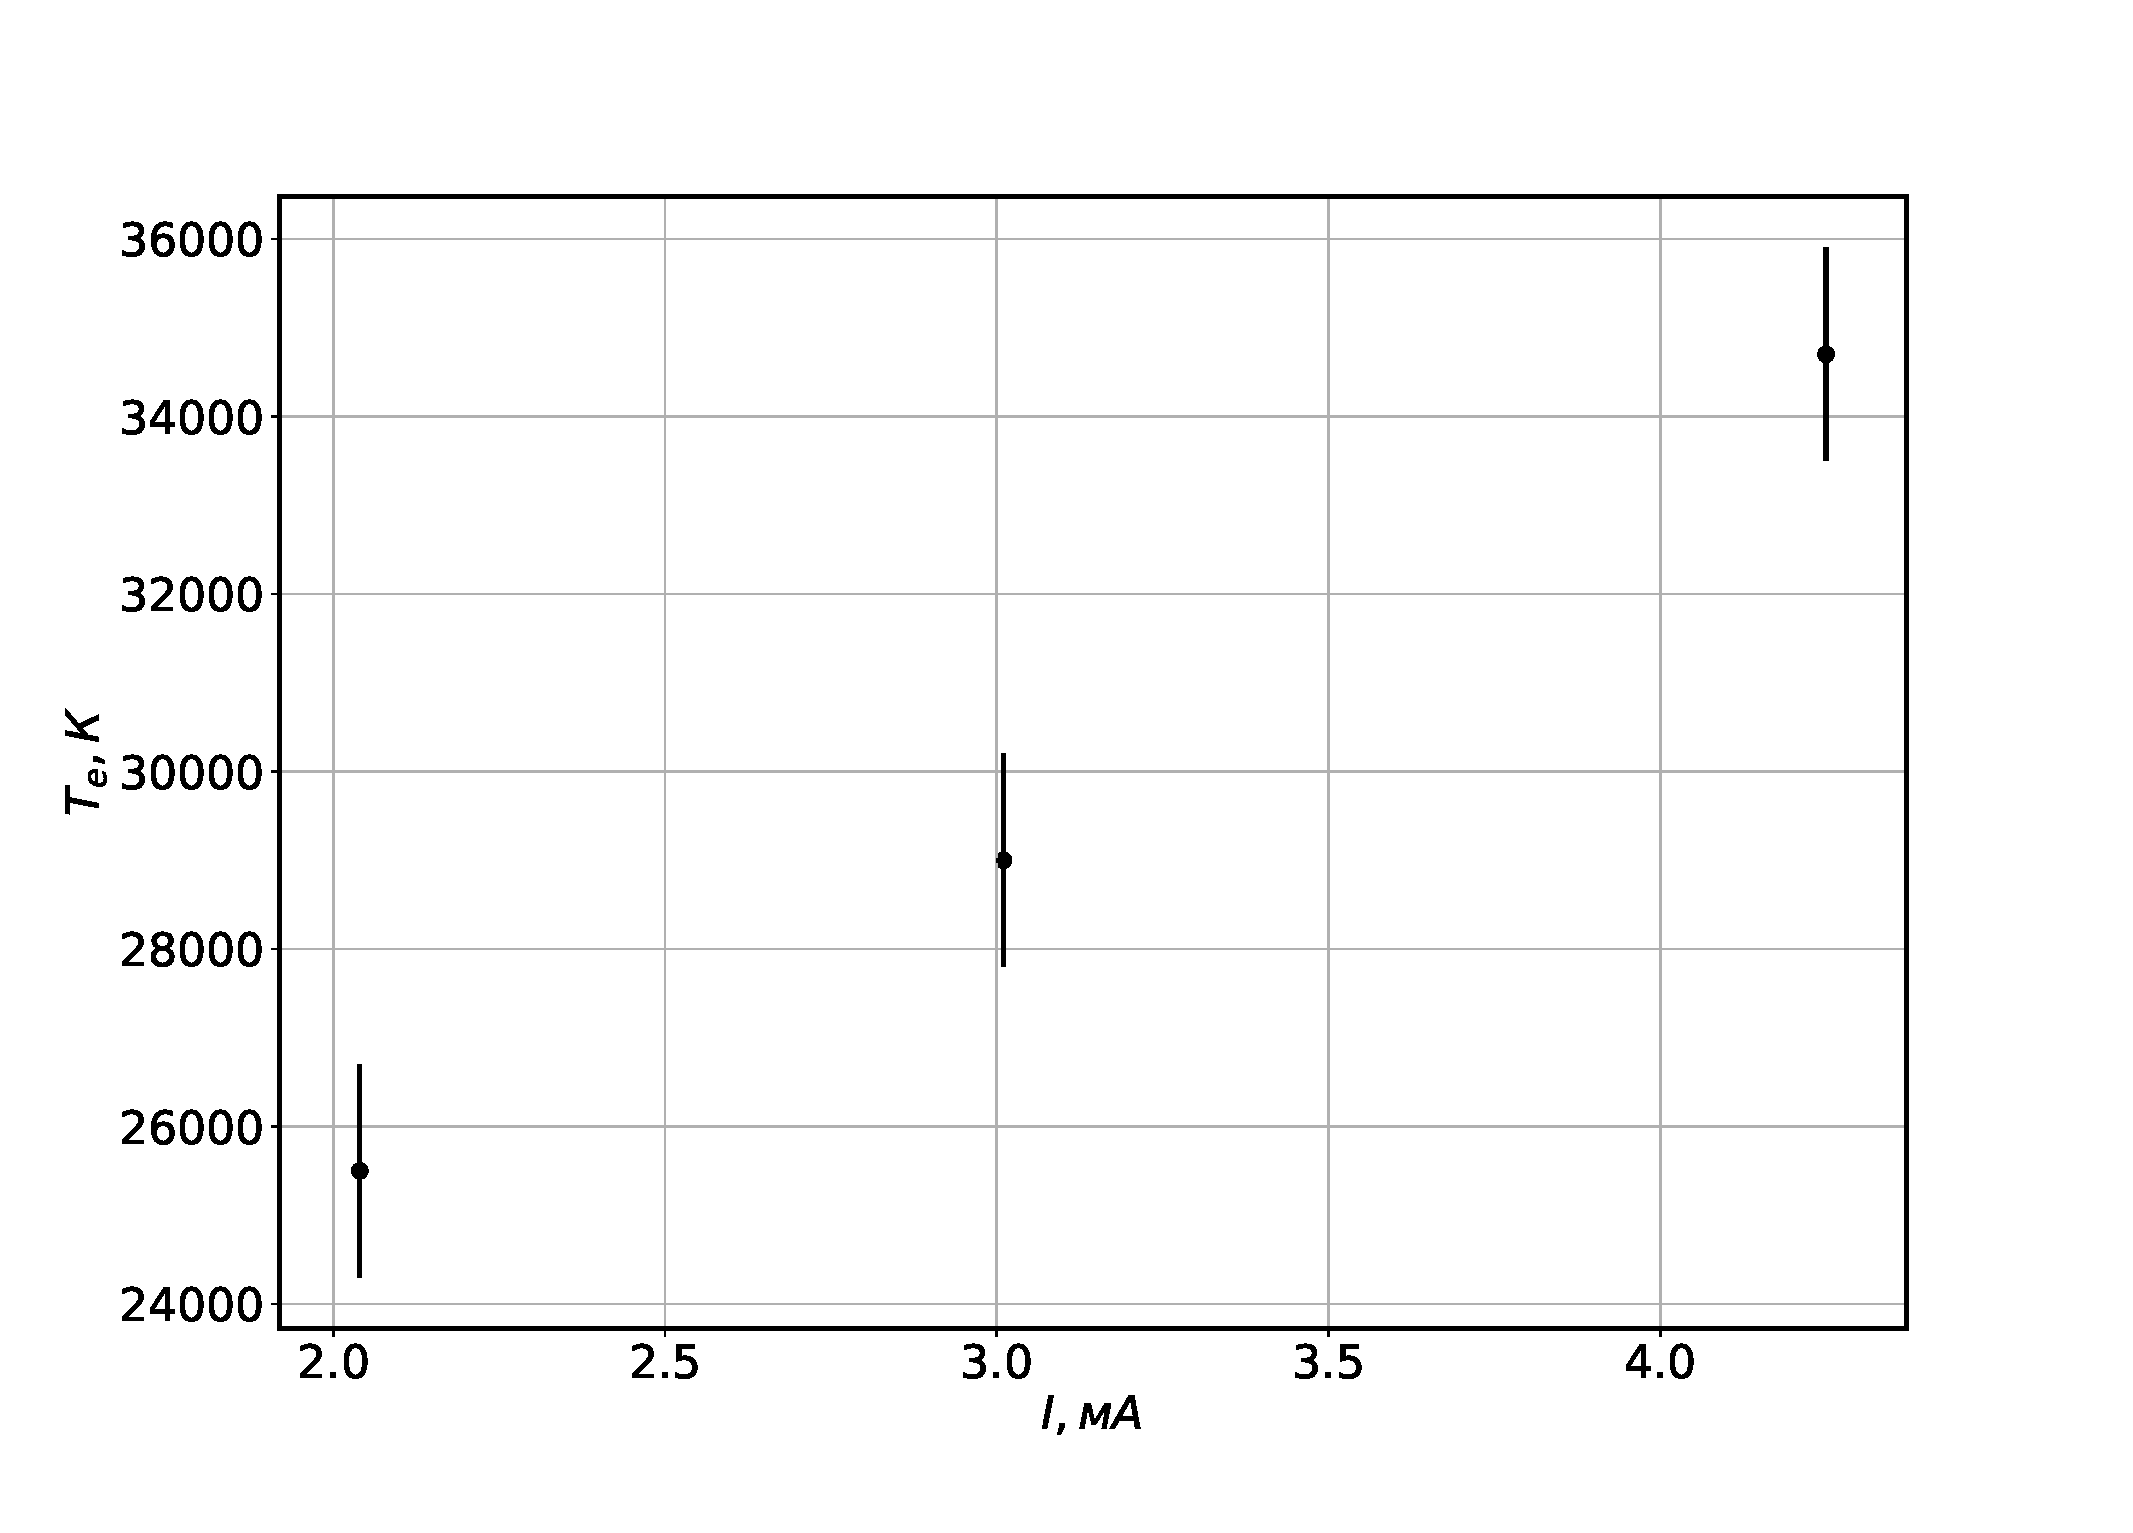
\includegraphics[width=0.8\textwidth]{TeI.eps}
	\caption{График температуры электронов $T_e$ от тока в плазме $I$.}
	\label{fig:TeI}
\end{figure}

\begin{figure}[H]
	\centering
	\includegraphics[width=0.8\textwidth]{neI.eps}
	\caption{График концентрации электронов $n_e$ от тока в плазме $I$.}
	\label{fig:neI}
\end{figure}

\begin{table}
	\centering
	\begin{tabular}{|r|r|r|r|r|r|}
		\hline
		$I_1$, мкА & $U_1$, В & $I_2$, мкА & $U_2$, В & $I_3$, мкА & $U_3$, В \\ \hline
		52,4       & 25,0     & 41,4       & 25,0     & 41,4       & 25,0     \\ \hline
		52,7       & 22,0     & 41,4       & 22,0     & 41,4       & 22,0     \\ \hline
		53,2       & 19,0     & 41,8       & 19,0     & 41,8       & 19,0     \\ \hline
		53,5       & 16,0     & 42,0       & 16,0     & 42,0       & 16,0     \\ \hline
		54,1       & 13,0     & 42,3       & 13,0     & 42,3       & 13,0     \\ \hline
		56,0       & 10,0     & 43,1       & 10,0     & 43,1       & 10,0     \\ \hline
		58,9       & 8,1      & 44,5       & 8,0      & 44,5       & 8,0      \\ \hline
		65,7       & 6,0      & 47,7       & 6,1      & 47,7       & 6,1      \\ \hline
		76,4       & 4,1      & 54,3       & 4,0      & 54,3       & 4,0      \\ \hline
		93,7       & 2,0      & 64,3       & 2,0      & 64,3       & 2,0      \\ \hline
		109,3      & 0,5      & 74,5       & 0,5      & 74,5       & 0,5      \\ \hline
		53,4       & 25,0     & 42,3       & 25,0     & 42,3       & 25,0     \\ \hline
		53,8       & 22,0     & 42,7       & 22,0     & 42,7       & 22,0     \\ \hline
		53,7       & 19,0     & 42,8       & 19,0     & 42,8       & 19,0     \\ \hline
		54,1       & 16,0     & 43,0       & 16,0     & 43,0       & 16,0     \\ \hline
		55,0       & 13,0     & 43,3       & 13,1     & 43,3       & 13,1     \\ \hline
		57,1       & 10,0     & 44,2       & 10,0     & 44,2       & 10,0     \\ \hline
		61,0       & 8,0      & 46,0       & 8,1      & 46,0       & 8,1      \\ \hline
		68,3       & 6,0      & 49,7       & 6,0      & 49,7       & 6,0      \\ \hline
		80,2       & 4,0      & 56,3       & 4,1      & 56,3       & 4,1      \\ \hline
		98,0       & 2,0      & 66,7       & 2,0      & 66,7       & 2,0      \\ \hline
		113,4      & 0,5      & 76,5       & 0,5      & 76,5       & 0,5      \\ \hline
	\end{tabular}
	\caption{Вольт-амперные характеристики двойного зонда для различных токах
		в разряде. $U_1, I_1$ --- для тока $I = 4,25$ мА, $U_2, I_2$ --- для тока $I = 3,01$ мА,
		$U_3, I_3$ --- для тока $I = 2,04$ мА  }
	\label{tab:2}
\end{table}
\section*{Выводы}
Исследована вольт-амперная характеристика газового разряда. Получены вольт-амперных характеристики 
двойного зонда, помещённого в газовый разряд при различных токах в разряде. Определены основные харастеристики плазмы. 
На основе подученных данных сделан вывод о том, что плазму в газовом разряде можно считать идеальной ($N_D \gg 1$).


\section*{Использованная литература}
\begin{thebibliography}{9}
	\bibitem{LabBook}
	Лабораторный практикум по общей физике, Том 2, под редакцией А. Д. Гладуна
\end{thebibliography}
\end{document}